\documentclass[11pt]{amsart}

% Standard letter size paper with 1inch margins
\usepackage[letterpaper, margin=1in]{geometry}
\usepackage{booktabs} % For better looking tables
\usepackage{xcolor}
\usepackage{pifont}

% Useful packages 
\usepackage{amsmath, amssymb, amsthm, amsaddr}
\usepackage{enumerate, subcaption, graphicx, hyperref}
\usepackage{algorithm}
\usepackage{algpseudocode}
\usepackage{cite}
\usepackage{bm}

\newcommand{\I}{\mathrm{i}}
\DeclareMathOperator{\E}{e}

\title{AMATH 582: Homework 3}
\author{Hunter Lybbert} % first and last name

\address{Applied Mathematics Department, University of Washington, Seattle, WA 
\\ \texttt{hlybbert@uw.edu}}

\date{\today} % you can also just type the date instead of "\today"

\begin{document}

\maketitle

\begin{abstract}
    In this report we convey the results of our survey of supervised machine learning algorithms.
    The MNIST digits dataset was used as a demo task to compare the performance for each of the supervised ML algorithms. We made use of the Ridge Regression Classifier, K-Nearest Neighbors, and Linear Discriminant Analysis. As well as other methods not discussed in class such as Random Forest Classifier and a Gradient Boosted Classifier. Descriptions of the methods, their implimentations, and results are given.
\end{abstract}

\section{Introduction and Overview}\label{sec:Introduction}
In this report we solidify our understanding of basic machine learning concepts by way of a simple supervised learning task, digit recognition.
We are using the MNIST data set.
The data set was provided to us already split into training and test sets.
The data is from \href{http://yann.lecun.com/}{Yann Lecun} and was provided to us through google drive to download.

The basic setup for supervised machine learning is given a collection of $N$ data points with labels in classification or target values in a regression setting $$\big\{(\bm{x_0}, y_0), (\bm{x_1}, y_1), ..., (\bm{x_{N-1}}, y_{N-1})\big\}.$$
We can also organize the data in terms of a data matrix $X$ and a vector of target values or class labels $\bm y$.
We then are looking for a function $f$ which takes in the training data and most accurately predicts the target values or class labels, written in optimization form we are looking for the following
$$f_{MLE} = \underset{f}{\rm argmin } \frac 1 {2 \sigma^2}|| f(X) - \bm y ||_2^2$$
where $\sigma^2$ is the variance of the normally distributed error terms $\epsilon \sim \mathcal N (0, \sigma^2)$ defined by $\epsilon_i = y_i - f(x_i)$.
So said another way we are trying to minimize our errors in the classification task.
This is the fundamental overview of what we are doing in this report.
The selection of class of functions $f$ to be considered to solve the problem is where our analysis comes into play. We evaluate the performance of a Ridge Regression Classifier, K-Nearest Neighbors, and Linear Discriminant Analysis models as well as other methods not discussed in class such as Random Forest Classifier and a Gradient Boosted Classifier on this digit classification task.

I would like to acknowledge the critical use of the following packages in our analysis.
Namely, Matplotlib was used to create all plots and animations \cite{Hunter:2007}.
Additionally, Scikit-learn was the primary source of using the PCA algorithm and other classification methods \cite{scikit-learn}.

\begin{figure}[h]
	\centering
	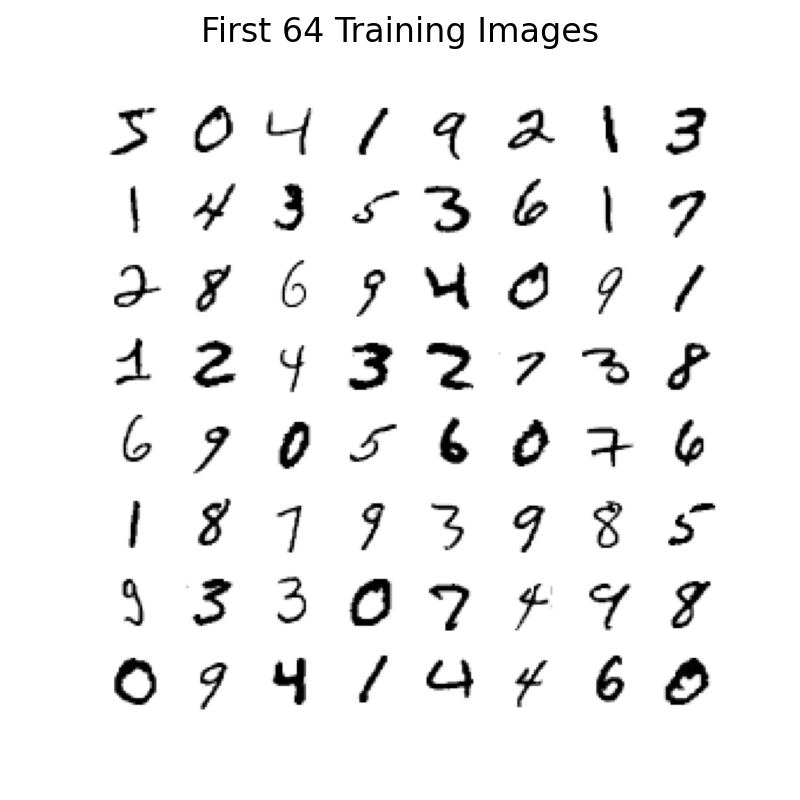
\includegraphics[width=.5\textwidth]{../visualizations/first_64_training_images.png}
 	\caption{ As an insight to the problem at hand I have visualized the first 64 training images.
	Not included in this report but available on my GitHub are animated visualizations of all training samples for a given digit. Something interesting that this revealed is that many of the training samples for the digit 2, us the curly circular style in the lower left hand corner of the symbol. This is notable because that makes a starker difference between 2 and 7 than we would expect. This could explain why 2 and 7 are easier to diliminate than we assumed. }\label{fig:f3}
\end{figure}

\section{Theoretical Background}\label{sec:theory}

In classifying our digit dataset we are considering data points which are 28x28 images therefore each datapoint has 784 input variables and from that information we are trying to predict the class labels.
Many machine learning algorithms will degrade in training time and performance with too many input features, therefore we consider using PCA as a data preprocessing step.
For a theoretical background and underpinning of PCA, please see my report 02.

In order to decide how many PC modes we needed to project our data down to in order to still preserve 85\% of the energy or information of the data we used the following energy metric
$$E = ||A||_F^2 = \sum_{j=0}^{ {\rm min}(m,n)} \sigma_j^2$$
where $\sigma_j$ are the singular values of the $(m,n)$ matrix $A$.
This is the total energy of the matrix $A$.
So when trying to calculate pc modes needed to preserve 85\% of total energy we calculate the partial cumulative sum over the singular values and normalize by dividing by the total energy $E$.
Once we reach 85\% we stop and that is the number of pc modes we need. Please see \ref{fig:f1} for a visualization of this process as we applied it.
Talk about PCA and how we determine the number of PC modes to project down to.

After projecting our training and test data to 59 pc modes space, we are ready to train various models using the different machine learning algorithms and compare their results.
Before discussing the results of each algorithm I will outline the various methods we utilize in this analysis.

\subsection{Ridge Regression (Classification)}
Recall our basic supervised machine learning setup where we are trying to find a function $f$ to take in the data $X$ and approximate as close as possible the values of the targets or labels $\bm y$.
Regression assumes the function $f$ takes the form 
$$f(X_{i,:}) = \beta_0 + \sum_{j=1}^d \beta_j X_{i,j}$$
where $X_{i,:}$ is the $i$th row of X which is the $i$th data point and $d$ is the dimension of our data.
This can thus be formulated as an optimization problem
$$ \beta_{MLE} = \underset{ \beta} {\rm argmin} \frac 1 {2 \sigma^2} || A\beta - y||^2$$
where A is the data matrix $X$ with a column of 1's prepended to the left side of the matrix $X$, this corresponds to the coefficient $\beta_0$.
This has an explicit solution which is $\beta_{MLE} = (A^TA)^{-1}A^Ty$

One challenge of this method is that inverting $A^TA$ can be expensive or infeasible if our data results in a singular matrix.
A method of mitigating this is called regularization.
We will specifically highlight here what is often known as L2 regularization.
This alters our original problem to the form
$$ \beta_{MLE} = \underset{ \beta} {\rm argmin} \frac 1 {2 \sigma^2} || A\beta - y||^2 + \frac \lambda 2 ||\beta||_2^2$$

where $\lambda$ is a learnable parameter which controls our tolerance for large magnitude weights in $\beta$.
The new resulting exact solutions is $\beta_{MLE} = (A^TA + \sigma^2\lambda I)^{-1}A^Ty$ which is now always guaranteed to be invertible.
I will not get into the proof of this, but it can be seen in class notes as well as online.

Finally, it is important to highlight how this regression based method is converted into a classification method by sklearn by assigning a value to each class and then trying to predict those values using regression.

Due to the space constraint in this report, the following algorithms will be treated much more briefly.

\subsection{K Nearest Neighbors (KNN)}

The k-nearest neighbor algorithm is a method which looks for the $k$ closest points to the data point which we are trying to classify and each of those k nearest neighbors vote with their own class label as to what the unknown point should be classified as. The most common class label in the $k$ neighbors wins out and is used to classify the unknown data point.

\subsection{Linear Discriminant Analysis }
A variation on the singular value decomposition and principal component analysis.
We will return to this and treat it in more detail if time permits.

\subsection{Random Forest Classifier}
A random forest classifier is a really a collection of classifiers called Decision Trees which each are trained and vote what they think the given datapoint aught to be classified as and the majority vote wins.
So we will primarily establish the theoretical background for the Decision Tree.
The basic process of generating a decision tree is deciding how to split the tree at a given step.
The decision tree wants to make a split in the data for example determining if a given datapoint $x_i$ has a value above or below a decided threshold for feature $j$.

In a more concrete example, suppose we had a different dataset with features such as students height, the total calories they burn a day, and their average body temperature, to try and classify students into two groups such as  high and low metabolism.
When the decision tree algorithm is considering what feature to split on and what value to split it at, it will consider all possible splits and choose the one that increases the class separation the most in the next step.

There are various metrics which can be used to make this split decision, the interested reader can refer to them in any machine learning or statistical learning text. A more important point is that a random forest classifier is a collection of these decision trees all casting their vote for which class the unknown datapoint should be classified as.

\subsection{Gradient Boosting Classifier}
Gradient Boosting is an amazing variation on a decision tree or random forest classifier.
Rather than training many classifiers to perform the same task in slightly different ways and all casting their vote we rather train one tree evaluate it's error and then train another tree to try and predict the error of the first one (in order to correct for the error).
Subsequent trees are trained until we reach the max number of trees we want to train or a min threshold of accuracy is reached.
This is admittedly not well suited for the problem of classification in our case, but is a powerful algorithm and was worth checking out its performance. \\

Both Gradient boosting and random forest take a lot more time to train since they are actually training sometimes hundreds of submodels. \\

\section{Algorithm Implementation and Development}\label{sec:algorithms}
A few key things to highlight in our actual implementation here. We considered performing a Standard Scaling (0 mean centering and scaling to unit variance) preprocessing step on our data, however, it seemed not necessary in our case.
Typically it is more important when datapoints were measured in different units which are orders of magnitude different from one another.
In our case each feature is just a pixel which takes on an integer value between 0 and 255.
We do however, perform PCA as a preprocessing step. \\

Furthermore, I want to highlight the importance of cross validation in our model training.
Whenever we train a model we hold out a test set to evaluate our model's performance.
Additionally, at times we might want to evaluate things like possible overfitting or hyper parameter tuning within the training process.
Specifically, $k$-fold cross validation is when we take our training set and break it into $k$ subsets using some predetermined algorithm (could be random subsets or some strategic method).
Then for each of the $k$ subsets we train a model on the other $k-1$ subsets and validate on the held out $k$th subset.
This gives us $k$ model's to compare validation accuracies against each other.

Again, due to space constraints I will not be discussing more details of implementation other than the fact that I utilized sklearn to setup the models and their preprocessing steps into pipeline objects which encapsulate the end to end process of preprocessing and training a model into one object.
It is an important tool in machine learning engineering.

\begin{figure}[h]
	\centering
	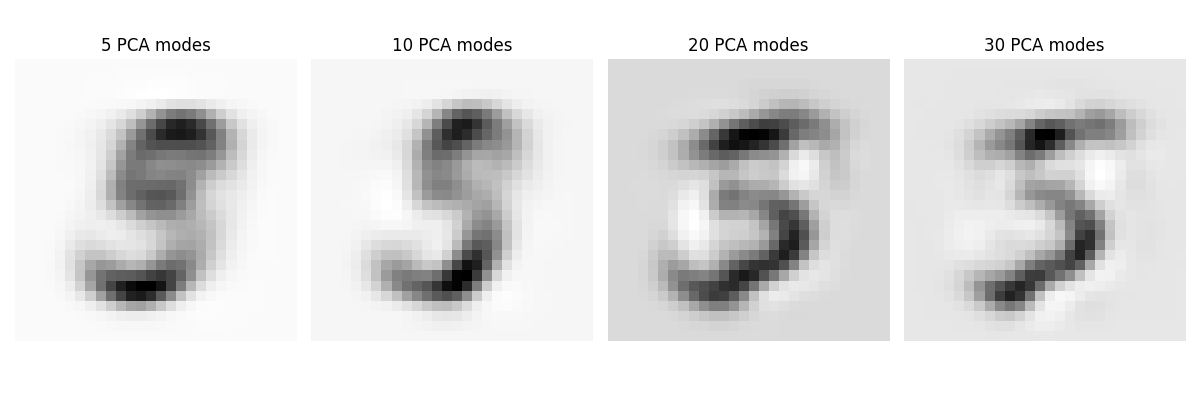
\includegraphics[width=.5\textwidth]{../visualizations/digit_reconstruction.png}
 	\caption{ An analysis of how much information or energy is retained in our data matrix given a certain number of components are used in the PCA transformation.
	We have visualized the reconstructed images after they've been projected to k-pc mode space and inversed to the original space.
	We can see the 59 pc modes really do retain a large amount of information (85\% as calculated using the cumulative energy)}\label{fig:f0}
\end{figure}

See Figure \ref{fig:f1} for the visuals described.

\begin{figure}[h]
    \centering
    \begin{subfigure}{0.4\textwidth}
        \centering
        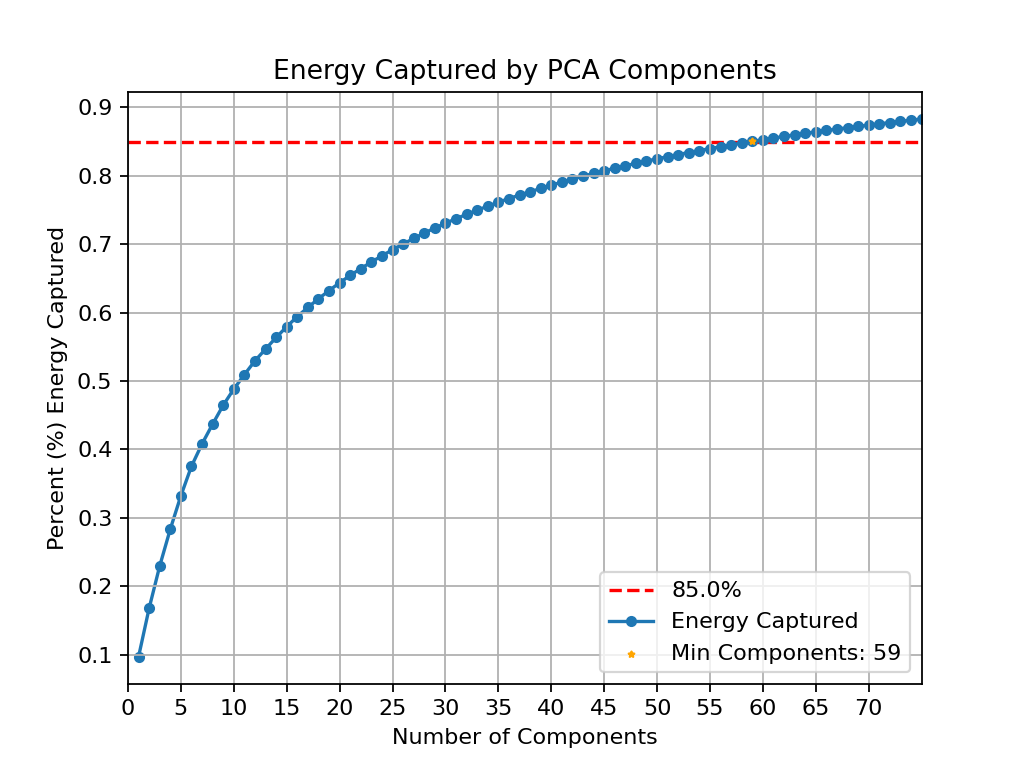
\includegraphics[width=\textwidth]{../visualizations/energy_by_components.png}
        \label{fig:image1}
    \end{subfigure}
    \caption{ This is the percentage of Total Energy which is preserved by projecting our digit images into a given number of pc modes. 
    We were tasked to calculate the minimum number of pc modes needed to be kept in order to retain 85\% of the total energy or information from the original image.
    As displayed with the orange star overlayed on the plot, the minimum number of pc components needed are 59.}
    \label{fig:f1}
\end{figure}

\section{Computational Results}\label{sec:results}

To be concise, notice in table \ref{tab:tab0} we have displayed the results of the binary classification using ridge regression.
We expected for 2 and 7 to be harder to distinguish, however by their test accuracy it actually performed better on it than 3 and 8. 
One possible reason for this is that many of the samples of 2 use the curly circular style 2 in the lower left corner of the symbol, which would make 2 and 7 more distinct than we typically expect. 
Furthermore, perhaps in the 59 pc mode space 3 and 8 get more confused and hazy due to their similarity overall.
Nevertheless, we are talking about minuscule differences in accuracies.
All of the models received A grades on an academic scale and their differences were subtle.
Furthermore, on the multi-class classification task with all digits there quickly became a better model.
See in table \ref{tab:tab1} that KNN performed best on the multi-class classification.
RidgeClassifierCV was used to determine that using an alpha or ($\lambda$) of 10 was optimal.

\begin{table}[h]
    \centering
    \begin{tabular}{|l|c|c|c|c|} % 'l' for left-aligned, 'c' for center-aligned columns
        \hline
        \textbf{Classifier} & \textbf{Digits Used} & \textbf{Train Accuracy} & \textbf{Test Accuracy} & \textbf{CV Score} \\ 
        \hline
        Ridge Classifier & 1 and 8 & 0.965  & 0.980 & 0.963 $\pm$ 0.00281 \\
        \hline
        Ridge Classifier & 3 and 8 & 0.961  & 0.964 & 0.959 $\pm$ 0.00590 \\
        \hline
        Ridge Classifier & 2 and 7 & 0.981  & 0.973 & 0.981 $\pm$ 0.00226 \\  
        \hline
    \end{tabular}
    \caption{The performance of RidgeClassifier on different binary digit classification problems. First evaluated on the task of distinguishing between 1 and 8, followed by 3 and 8, then finally 2 and 7.}
    \label{tab:tab0}
\end{table}

\begin{table}[h]
    \centering
    \begin{tabular}{|l|c|c|c|} % 'l' for left-aligned, 'c' for center-aligned columns
        \hline
        \textbf{Classifier} & \textbf{Train Accuracy} & \textbf{Test Accuracy} & \textbf{CV Score} \\ 
        \hline
        Ridge Classifier & 0.845  & 0.856 & 0.844 $\pm$ 0.00997 \\  
        \hline
        K-nearest Neighbors & 0.986 & 0.976 \textcolor{red}{\ding{72}} & 0.975 $\pm$ 0.00109 \\
        \hline
        Linear Discriminant Analysis & 0.866 & 0.875 & 0.865 $\pm$ 0.00870 \\  
        \hline
        Random Forest Classifier & 0.998 & 0.947 & 0.942 $\pm$ 0.00407 \\  
        \hline
        Gradient Boosting Classifier & 0.939 & 0.928 & 0.918 $\pm$ 0.00554 \\  
        \hline
    \end{tabular}
    \caption{The performance of each model on the full digit recognition task, aka multi-class classification of digits.
    Using the performance on the test set as our selection metric, I would conclude that K-nearest Neighbors performed best on this classification task.}
    \label{tab:tab1}
\end{table}


\begin{figure}[h]
	\centering
	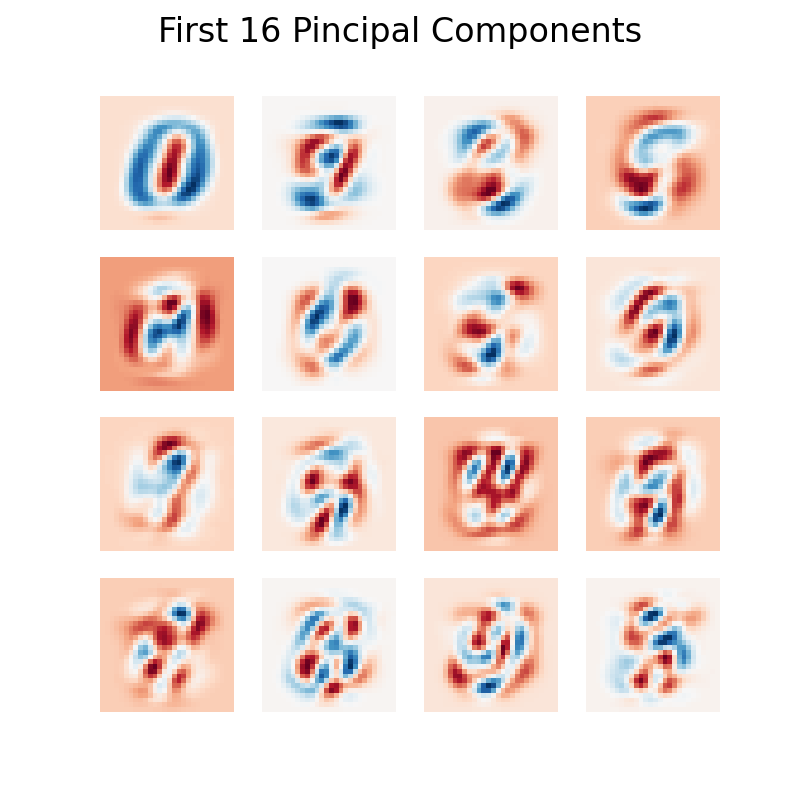
\includegraphics[width=.5\textwidth]{../visualizations/first_16_pincipal_components.png}
 	\caption{ Here we have visualized the first 16 pc modes. These represent a basis for the 16 pc mode space where you can represent the image data as a linear combination of these modes.}\label{fig:f2}
\end{figure}

\section{Summary and Conclusions}\label{sec:conclusions} 
In summary, the digit classification task is a someone uninteresting use case since the models perform so well generally.
However, because it is an easy to understand application it allowed us to learn more about how these various algorithms compare to one another in terms of training times and performance on the test set.
Additionally, it provided a great opportunity to dig into how to use sklearn's built in methods for these various machine learning algorithms.

\section*{Acknowledgements}

The author is thankful to Jaxon Tuggle, Hailey Sparks, Anja Vogt, Jade Glaister, and Nate Ward for offering regular feedback and counsel when interpreting results and clarifying the implications and merits of different classifiers.
We would also like to thank Professor Eli Shlizerman for carefully instructing us in class.

\bibliographystyle{abbrv}
\bibliography{references_hw3} % make sure this matches the .bib file for your corresponding document. You also have to maintain your references in the .bib file 

\end{document}
